% **********************************************************************
% Copyright 2023 Aleksander GRM

% Author: Aleksander GRM @fpp.uni-lj.si
% Description: This is an unofficial report template I made from scratch. 
%              Feel free to use it, modify it, and share it.
% Version: 1.0
% Date: 02/05/2024
% URL: https://github.com/as-grm/latex_templates
% **********************************************************************


% ******************
% *** page style ***
%
% *** single side page ***
\documentclass[12pt]{article}
%
% *** two side pages ***
%     must also use correct page margins and fancyhdr
%
%\documentclass[11pt,twoside]{article} % If needed twosided
% ******************


\usepackage[pdftex]{hyperref} % hyperref
\usepackage[utf8x]{inputenc}  % utf-8 support 
\usepackage[T1]{fontenc}      % necessary


% ******************************************
% *** hyper references must be set first ***
% ******************************************
%
\hypersetup{
	colorlinks = true,
	linkcolor = {red!50!black},
	citecolor = {blue!50!black},
	urlcolor = {blue!80!black}
}



% ************************
% *** Language support ***
% ************************
%
\usepackage[slovene]{babel}
%\usepackage[english]{babel}
% ************************



% *** show labels ***
% \usepackage{showlabels}

% *********************
% *** Paper margins ***
% *********************
%
\usepackage{vmargin}
%\setmarginsrb{leftmargin}{topmargin}{rightmargin}{bottommargin}
%{headheight}{headsep}{footheight}{footskip}
\setpapersize{A4}
% twoside
%\setmarginsrb{30mm}{15mm}{20mm}{15mm}{10mm}{10mm}{10mm}{15mm}
% oneside
\setmarginsrb{25mm}{15mm}{25mm}{15mm}{10mm}{10mm}{10mm}{15mm}


%%%%%%%%%%%%%%%%%%%%%%%%%%%%%%%%%%%%%%%%%%%%%%%%%%%%%%%%%%%%%%%%%%%%%%%%%%%%%%%
% DODATNE DEFINICIJE
%%%%%%%%%%%%%%%%%%%%%%%%%%%%%%%%%%%%%%%%%%%%%%%%%%%%%%%%%%%%%%%%%%%%%%%%%%%%%%%

% naložite dodatne pakete, ki jih potrebujete
\usepackage{algpseudocode}  % za psevdokodo
\usepackage{algorithm}      % za algoritme
\floatname{algorithm}{Algoritem}
\renewcommand{\listalgorithmname}{Kazalo algoritmov}


\usepackage[numbers]{natbib}
\usepackage{parskip}
\usepackage{graphicx}
\usepackage{xcolor}
\usepackage{subfigure}
\usepackage{multicol}
\usepackage{mathtools}
\usepackage{amsmath,amsthm,amssymb,latexsym}
\usepackage{empheq, nccmath}
\usepackage[many]{tcolorbox}
\usepackage{siunitx}
\usepackage{datetime}
\usepackage{fancyhdr}
\usepackage{enumitem} % oklje za naštevanje

% okolja za lepe tabele
\usepackage{booktabs} % fancy tables
%\usepackage[rgb]{xcolor}
%\selectcolormodel{natural}
\usepackage{ninecolors}
\selectcolormodel{rgb}
\usepackage{tabularray}
%
% registered - \textregistered
% copyright  - \textcopyright
\usepackage{textcomp}

%
\usepackage[all,knot]{xy}
\xyoption{arc}
\usepackage{multimedia}
\usepackage{setspace}
\usepackage{listings}
\usepackage{textcomp}
\usepackage{bm}
\usepackage{xfrac}
\usepackage{tikz}
\usepackage{cancel}
\usetikzlibrary{shadings}

% deklarirajte vse matematične operatorje, da jih bo LaTeX pravilno stavil
% \DeclareMathOperator{\conv}{conv}
% na razpolago so naslednja matematična okolja, ki jih kličemo s parom
% \begin{imeokolja}[morebitni komentar v oklepaju] ... \end{imeokolja}
%
% definicija, opomba, primer, zgled, lema, trditev, izrek, posledica, dokaz

% za številske množice uporabite naslednje simbole
\newcommand{\R}{\mathbb R}
\newcommand{\N}{\mathbb N}
\newcommand{\Z}{\mathbb Z}
% Lahko se zgodi, da je ukaz \C definiral že paket hyperref,
% zato dobite napako: Command \C already defined.
% V tem primeru namesto ukaza \newcommand uporabite \renewcommand
\newcommand{\C}{\mathbb C}
\newcommand{\Q}{\mathbb Q}

%
% *** Matlab
%
\usepackage[framed,numbered]{matlab-prettifier}

%
% *** Caption to be boldface ***
%
\usepackage{caption}
\captionsetup[figure]{labelfont=bf}

%
% *** Numbered environment ***
%
%\newenvironment{naloga}[1][]{\noindent \textbf{Naloga} }{\medskip}
\newenvironment{primer}[1][]{\noindent \textbf{Primer.}  }{\medskip}
\newenvironment{resitev}[1][]{\noindent \textbf{Rešitev.}  }{\medskip}

%
% *** Examples ***
%
\theoremstyle{definition}
\newtheorem{exmp}{}[section]
\newtheorem{naloga}{Naloga}[section]

% 
% *** Literatura ***
%
\newcommand{\vkljucibibliografijo}[1]{%
	\cleardoublepage
	\singlespacing
	\addcontentsline{toc}{section}{Literatura}
	\bibliographystyle{plainnat}
	\bibliography{#1}
}

%
% *** Fancy header ***
%
\pagestyle{fancy}
\fancyhf{}
\lhead{\textsc{Navodila \LaTeX}}
\chead{}
\rhead{\textcopyright 2025 \textsc{Avtorji}}
\cfoot{\thepage}


%%%%%%%%%%%%%%%%%%%%%%%%%%%%%%%%%%%%%%%%%%%%%%%%%%%%%%%%%%%%%%%%%%%%%%%%%%%%%%%
% ZAČETEK VSEBINE
%%%%%%%%%%%%%%%%%%%%%%%%%%%%%%%%%%%%%%%%%%%%%%%%%%%%%%%%%%%%%%%%%%%%%%%%%%%%%%%

\begin{document}
\pagenumbering{roman}

%%%%%%%%%%%%%%%%%%%%%%%%%%%%%%%%%%%%%%%%%%%%%%%%%%%%%%%%%%%%%%%%%%%%%%%%%%%%%%%%%%%%%%%%%
\thispagestyle{empty}

    \begin{center}
	    
\includegraphics[height=6cm]{figs/fpp_logo_uradni.pdf}\\[2.0 cm]
	    
		\rule{\linewidth}{1 mm} \\[7mm]
		{ \huge \bfseries Poročilo}\\[4mm]
		\rule{\linewidth}{1 mm} \\[4mm]
		\doublespacing
		{ \Large \bfseries Navodila pisanja zaključnega dela in poročil v \LaTeX okolju}\\[1mm]
		\singlespacing
		\rule{\linewidth}{1 mm} \\[3cm]
		
		\begin{flushleft} \large
			\emph{Avtorji:}\\[3mm]
			\hspace{1cm}\textsc{D. Žagar, A.S. Grm in F. Dimc}\\[1mm]
		\end{flushleft}
		
		\vfill
		
		{\large \today}\\[1cm]
	\end{center}
	
%%%%%%%%%%%%%%%%%%%%%%%%%%%%%%%%%%%%%
\newpage
\thispagestyle{plain}

\tableofcontents


%%%%%%%%%%%%%%%%%%%%%%%%%%%%%%%%%%%%%%
\newpage
\pagenumbering{arabic}
\setcounter{page}{1}

% *********************
% *** Novo poglavje ***
% *********************
\newpage
\section{Uvod}
\label{sec:Uvod}

Pričujoča navodila bodo kažipot za študente na \textsc{UlFpp}, ki bodo svoja poročila in naloge pisali v \LaTeX okolju. 

\LaTeX je okolje, ki ga uporablja večina najbolj znanih tehničnih univerz za pisanje poročil in zaključnih nalog in s tem tudi \textsc{FPP} kot tehnična fakulteta, je edinstveno okolje za procesiranje teksta. Znotraj imamo skoraj neomejene možnosti formatiranja teksta. Predvsem je pravilo, tisto kar postavimo in vidimo, bo vedno tako.

Obdelava teksta potrebuje prevajalnik, ki si ga lahko namestimo na lastnem računalniku. Tako imamo različne sisteme

\begin{itemize}[nosep]
	\item MikTeX (\url{https://miktex.org}) je dostopen za vse operacijske sisteme, vendar se ga največ uporablja prav v Windows OS,
	\item TexLive (\url{https://www.tug.org/texlive}) je drugo tako splošno okolje, ki pa se ga največ uporablja v Linux OS in Mac OS,
	\item LaTeX projekt (\url{https://www.latex-project.org}) je spet tako splošno okolje za vse OS.
\end{itemize} 

Druga stvar je editor v katerem naj bi tekst urejali. Najbolj priporočamo prav TexStudio, imamo pa udi druga okolja

\begin{itemize}[nosep]
	\item TexStudio (https://www.texstudio.org)
	\item VisualStudio (\url{https://marketplace.visualstudio.com/items?itemName=James-Yu.latex-workshop})
	\item TexMaker (\url{https://www.xm1math.net/texmaker})
	\item TexPage (\url{https://www.texpage.com/})
	\item $\dots$
\end{itemize}

Vse tole si je potrebno inštalirati na lastnem računalniku. Če niste prevelik navdušenec nad tem, obstaja pa profesionalna spletna aplikacija, ki omogoča tudi brezplačno storitev. To je za začetek najbolje. To je spletna aplikacija OverLeaf (\url{https://www.overleaf.com}). Kar je lepota OverLeaf okolja je, da lahko dokument delite z drugimi, kot je na primer vaš mentor in s tem omogočite direktno vnašanje pripomb. Podpira tudi \emph{Review} način, kjer lahko sledite vsem popravkom in jih sprejemate, zavračate, komentirate in podobno.


% *********************
% *** Novo poglavje ***
% *********************
\newpage
\section{Postavitev delovnega \LaTeX okolja v OverLeaf aplikaciji}
\label{sec:Overleaf}

Spletno okolje OverLeaf je dosegljivo preko naslova \url{https://www.overleaf.com}. Tukaj se registrirate kot uporabnik in potem lahko kar pričnete z delom.

Ko ste enkrat registrirani, se vam odpre osnovno okno, kjer so prikazani vsi vaši projekti

\vspace*{5mm}
\begin{center}
	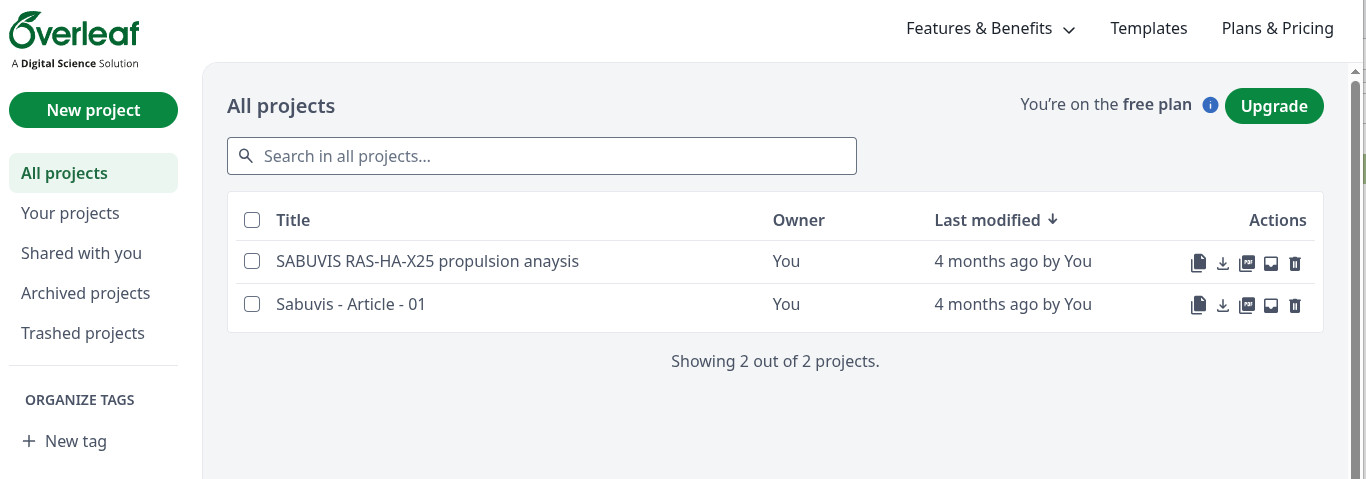
\includegraphics[width=\linewidth]{figs/overleaf_01.jpg}
\end{center}
\vspace*{5mm}

Kliknete na \texttt{New projekt} in ustvarite nov latex projekt. Ponudijo se vam različne možnosti, kjer je najbolje izbrati \texttt{Blank project} in uvozite predlogo FPP.

Uvažanje je enostavno, samo kliknete na ikono za upload

\vspace*{5mm}
\begin{center}
	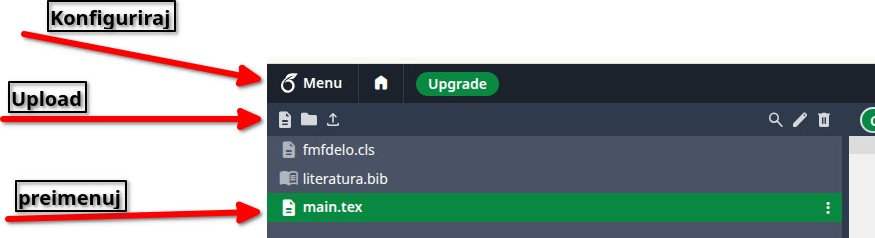
\includegraphics[width=0.6\linewidth]{figs/overleaf_02.jpg}
\end{center}
\vspace*{5mm}

in uvozite tri datoteke:

\begin{itemize}[nosep]
	\item \texttt{fpptemplate.cls}
	\item \texttt{literatura.bib}
	\item \texttt{main.tex}
	\item \texttt{sklep\_kzsz.pdf}
\end{itemize}

in naredite si še mapo \texttt{figs}, kamor boste nalagali slike. V naslednjem koraku preimenujte datoteko \texttt{main.tex} v \texttt{naloga\_ime\_priimek.tex}. Sedaj odprite datoteko

\texttt{naloga\_ime\_priimek.tex}

in pričnete lahko z delom.

%
\subsection{Nastavitve}

Preden pričnete resno z delom, dejte pogledat ali so vse nastavitve prave. Nastavitve preverite s klikom na \texttt{Menu}.

\texttt{Compiler} mora biti obvezno nastavljen na \texttt{pdfLatex}, drugače ne bo delalo. 

Pdf datoteko lahko snamete s serverja s kliko na \texttt{Menu} in potem na \texttt{PDF} ikono. Če kliknete na ikono \texttt{Source} boste lahko shranili vse razen pdf datoteke. Tole je ločeno, da lahko samo pdf shranite in ga pošljete nekomu drugemu.

Da bi mentorju omogočili pregledovanje, mu je potrebo dodati pravice. To storite tako, da vaš projekt delite (Share - zgoraj desno) in mu date pravice \texttt{Review} ali če mu zaupate v celoti pa pravice \texttt{Edit}.

V \texttt{Review} mode (klikinte zgoraj desno Review), se bodo pokazale pripombe mentorja. Tako lahko enostavno komunicirata z mentorjem, kaj je potrebno popraviti. 


% *********************
% *** Novo poglavje ***
% *********************
\newpage
\section{Osnovna navodila za pisanje v \LaTeX okolju}
\label{sec:Navodila}

% *** Podpoglavje ***
\subsection{Navodila za sestavo naloge}

Navodila za oblikovanje zaključnih del na Fakulteti za pomorstvo in promet Univerze v Ljubljani vsebujejo navodila, ki se nanašajo na:

\begin{itemize}[nosep]
	\item format del, postavitev strani in jezikovni pregled,
	\item tisk in oštevilčenje strani,
	\item oblika in velikost pisave,
	\item številčenje poglavji,
	\item predpisan format postavitve tabel, slik, enačb in prilog,
	\item dodajanje opomb v nogo,
	\item citiranje virov in seznam literature,
	\item oblikovanje,
	\item izjava kandidata,
	\item $\dots$	
\end{itemize}

V primeru, ko zaključno delo pišete v \LaTeX okolju, se vam ni potrebno ukvarjati z zgoraj naštetimi navodili. Preprosto, kopirate \LaTeX predlogo in pričnete s pisanjem.

Študentje si lahko o \LaTeX okolju veliko preberejo na naslednjih naslovih:

\begin{itemize}
	\item Dobra navodila v angleščini so \textit{The Not So Short Introduction to \LaTeX 2$\varepsilon$}\\
	\url{https://tug.ctan.org/info/lshort/english/lshort.pdf},
	\item Slovenska verzija zgornjega dokumenta je na voljo na naslovu\\ \href{https://users.fmf.uni-lj.si/plestenjak/vaje/latex/lshort.pdf}{https://users.fmf.uni-lj.si/plestenjak/vaje/latex/lshort.pdf}\\
	kjer imate še dodatna navodila na naslovu\\
	\href{https://users.fmf.uni-lj.si/plestenjak/vaje/latex/latex.htm}{https://users.fmf.uni-lj.si/plestenjak/vaje/latex/latex.htm}
	\item \textbf{OverLeaf} projekt z pomočjo na naslovu \url{https://www.overleaf.com/learn},
	\item in še mnoga ostala literatura. 
\end{itemize}

\texttt{OverLeaf} (\url{https://www.overleaf.com}) projekt omogoča urejanje latex dokumentov kar v spletni aplikaciji. Študent si naredi račun, naredi projekt, ga odpre in začne kar z delom pisanja v \LaTeX u.

V primeru, da se vam pojavi črn kvadratek na skrajni desni strani, latex sistem ni mogel pravilno narediti preloma vrstice in morate sami dodati ročno prelom vrstice, ki je dvojni backslash (\textbackslash\textbackslash).


% *** Podpoglavje ***
\subsection{Pravilna izbira programa in smeri}

V prvi vrstici \LaTeX datoteke, se nahaja ukaz

\texttt{\textbackslash documentclass[pomstr, tisk]{fppthesis}}

Če želimo izbrati ustrezen program in smer, imamo naslednje možnosti:

\textbf{Pomorstvo}
\begin{itemize}[nosep]
	\item \texttt{\textbackslash documentclass[pomnav, tisk]\{fppthesis\}}: Navtika -- 1. stopnja
	\item \texttt{\textbackslash documentclass[pomstr, tisk]\{fppthesis\}}: Pomorsko strojništvo\\
	-- 1. stopnja
	\item \texttt{\textbackslash documentclass[pom2, tisk]\{fppthesis\}}: Pomorstvo -- 2. stopnja
\end{itemize}

\textbf{Promet}
\begin{itemize}[nosep]
	\item \texttt{\textbackslash documentclass[promuni, tisk]\{fppthesis\}}: TPL -- 1. stopnja
	\item \texttt{\textbackslash documentclass[prompttl, tisk]\{fppthesis\}}: PTTL -- 1. stopnja
	\item \texttt{\textbackslash documentclass[prom22, tisk]\{fppthesis\}}: Promet -- 2. stopnja
\end{itemize}

Ko izberemo ustrezni študij, moramo samo pravilno izpolniti polja, ki so določena v delu označenem z besedo \textbf{METAPODATKI}. V metapodatkih morate izpolniti vsa polja s svojimi podatki. Tako se bodo ustrezno ustvarile vse prve strani.

V primeru, da bi radi dokument objavili online, izbrišete besedo \texttt{tisk} in tako se dokument prelevi v interaktivni brez praznih strani.

% *** Podpoglavje ***
\subsection{Sestavljanje poglavji}

Vsa poglavja se morajo začeti na novi strani. Novo stran postavimo z uporabo ukaza za prehod na novo stran \texttt{\textbackslash newpage}. Tako zapišemo novo poglavje

\begin{verbatim}
	% *********************
	% *** Novo poglavje ***
	% *********************
	\newpage
	\section{Novo poglavje}
	\label{sec:novo_poglavje}	
\end{verbatim}

Če želimo v poglavju narediti še podpoglavja lahko gnezdimo navzdol z uporabo ukazov

\begin{verbatim}
	\subsection{Pod poglavje}
	\subsubsection{Pod pod poglavje}
\end{verbatim}

in tako naprej. Vsakemu poglavju dodamo sidro (\texttt{label}), s katerim se lahko nato v tekstu sklicujemo, recimo, v poglavju \ref{sec:Navodila} smo zapisali navodila.

% *** Podpoglavje ***
\subsection{Izdelava tabel, vnos slike, enačbe in priloge}

Tabele in slike (stolpični, črtni, tortni, palični in raztreseni grafi, sheme, modeli, fotografije itd.) morajo biti zaporedno oštevilčene (npr. Tabela 1, Slika 3) in naslovljene. Naslov tabele je nad njo, levo poravnan. Naslov slike je pod njo, sredinsko poravnan. Formule v besedilu zaporedno številčimo tako, da ob desnem robu strani v oklepaju zapišemo zaporedno številko formule.

Če je tabela ali slika prevzeta iz literature, mora biti tik pod tabelo ali sliko natančno naveden vir (velikost pisave vira: 9; sredinska poravnava); če je formula prevzeta iz literature, mora biti v besedilu, ki se na formulo nanaša, naveden njen vir (kot je navedeno v poglavju 6. Citiranje, povzemanje in seznam uporabljene literature). 

Tabele, slike in formule morajo biti postavljene na mesta, kamor vsebinsko sodijo, hkrati pa morajo biti v besedilu omenjene tako, da se navede njihova številka (npr. glej tabelo \ref{tab:primer_tabele1}).


\subsubsection{Tabele}

Primer lepe formatirane tabele:

\begin{table}[h]
	\caption{Primerjava med tovornima pristaniščema Koper in Reka.}
	\vspace*{1mm}
	\label{tab:primer_tabele1}
	\begin{center}
		\begin{tblr}{colspec={l|rr},
				%width=0\textwidth,
				row{even} = {white,font=\small},
				row{odd} = {bg=black!10,font=\small},
				row{1} = {bg=blue!20,font=\bfseries\small},
				hline{1} = {1pt,solid,black!60},
				hline{2} = {1pt,solid,black!60},
				hline{Z} = {1pt,solid,black!60},
				rowsep=3pt
			}
			% *** začetek podatko ***
			& Pretovor & TEU    & TEU/dvigalo & m3 \\ 
			Koper  & 353,880  &	88,470 & 594         & 12 \\
			Rijeka & 168,777  &	42,194 & 328         &	6
			% *** konec podatkov ***
		\end{tblr}
	\end{center}
	\vspace*{1mm}
	\begin{flushright}
		Vir:(Beškovnik in Twrdy, 2009)
	\end{flushright}
\end{table}

V tabeli zapisujemo podatke v vrsticah, kjer posamezne stolpce ločimo z znakom "\&". Konec vrstice zaključimo z dvojnim back-slash znakom "\textbackslash\textbackslash".

Postavitev table na strani dosežemo s črko v oglatem oklepaju za \texttt{\textbackslash begin\{table\}}, kjer imamo možnosti

\begin{itemize}[nosep]
	\item \texttt{[h]} -- here ali tukaj, to je točno tam, kjer se nahaja med tekstom,
	\item \texttt{[t]} -- top ali zgoraj, tabelo namestimo na zgornji del strani. To je ponavadi najbolje,
	\item \texttt{[b]} -- bottom ali spodaj, tabelo postavimo na spodnji del strani.
\end{itemize}


\subsubsection{Slike}

Slike vnašamo zelo preprosto, kjer je okolje \texttt{figure}. Če le lahko naj bodo slike ali v \texttt{pdf} ali v \texttt{jpg} formatu.

\begin{figure}[h]
	\begin{center}
		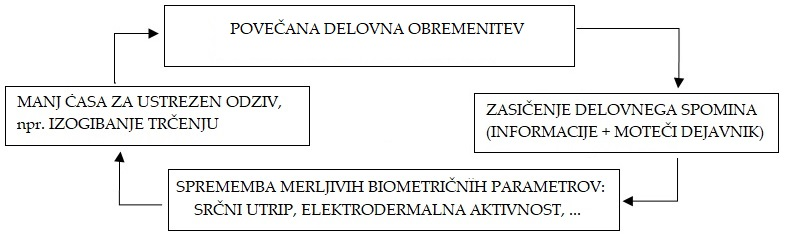
\includegraphics[width=0.7\linewidth]{figs/zasicenje.jpg}
	\end{center}
	\caption{Slika prikazuje nekaj, bla bla bla.}
	\label{fig:slika1}
\end{figure}

Širino slike določamo s faktorjem, ki stoji pred \texttt{\textbackslash linewidth}, kjer je \texttt{\textbackslash linewidth} širina okvirja teksta na strani. Enako se lahko na sliko preprosto sklicujemo v tekstu, recimo: Slika \ref{fig:slika1} prikazuje bla bla bla.

\subsubsection{Enačbe}

V \LaTeX okolju je pisanje enačb zelo preprosto. Za pisanje enačb lahko uporabimo več različnih okolji: \texttt{equation}, \texttt{equnarray}, \texttt{align}, \texttt{split}, \texttt{cases}, \texttt{array}, $\dots$ Vsako okolje ima svoje namen, kako izpisujemo enačbe.

Recimo, zelo veliko o pisanju v latexu si lahko študent pogleda na različnih lokacijah, ki smo jih navedli v začetku. V teh navodili so tudi lepo opisani postopki za pisanje enačb. Enako se enačbe številčijo s številkami, ki so v oklepajih. to je v latexu avtomatsko. Če ne želimo številke damo na koncu imena okolja zvezdico *.

Primeri:

\begin{equation}
	E = m \: c^2
	\label{eq:einstain}
\end{equation}

\begin{verbatim}
	\begin{equation}
		E = m \: c^2
		\label{eq:einstain}
	\end{equation}
\end{verbatim}

ali brez številke, če je enačba le pomožna kot del izpeljave

\begin{equation*}
	E = m \: c^2
\end{equation*}

\begin{verbatim}
	\begin{equation*}
		E = m \: c^2
	\end{equation*}
\end{verbatim}

Enačbe lahko enako kličemo po referenci, recimo Einštajn je zapisal nekaj zelo znanega v enačbi (\ref{eq:einstain}). V zgornjem primeru se je kot razmak med znaki uporabila kombinacija backslash in dvopičja (\texttt{\textbackslash :}).

\subsubsection{Pisanje algoritmov}
Za pisanje algoritmov sta na voljo okolji \texttt{algorithm} in \texttt{algorithmic} iz paketov \texttt{algorithm} in \texttt{algorithmix}, ki sodelujeta podobno kot \texttt{table} in \texttt{tabular}. Algoritmi plavajo med tekstom, enako kot slike in tabele, nanje se lahko tudi sklicujemo, kot prikazano v izvorni kodi in v algoritmu \ref{alg:metoda} (je na naslednji strani, ker se ga ne da prelomit). Sklicujemo se lahko tudi na pomembne vrstice, npr.\ na vrstico~\ref{alg:pomembna-vrstica}, ki predstavlja glavni del algoritma. Za primer pisanja algoritma se posvetujte s primerom v tem dokumentu, za bolj napredne primere uporabe, kot na primer razbijanje algoritma na več kosov, pa z (precej razumljivo) uradno dokumentacijo\footnote{\url{http://tug.ctan.org/macros/latex/contrib/algorithmicx/algorithmicx.pdf}}.

Če želite vključiti izvorno kodo nekega programa, priporočamo paket \texttt{minted}\footnote{\url{https://github.com/gpoore/minted}}.

\algnewcommand\algorithmicto{\textbf{to}}
\algnewcommand\algorithmicin{\textbf{in}}
\algnewcommand\algorithmicforeach{\textbf{for each}}
\algrenewtext{For}[3]{\algorithmicfor\ #1 $\gets$ #2\ \algorithmicto\ #3\ \algorithmicdo}
\algdef{S}[FOR]{ForEach}[2]{\algorithmicforeach\ #1\ \algorithmicin\ #2\ \algorithmicdo}

\begin{algorithm}[ht]
	\caption{Opis, ki ima enako funkcionalnost kot opis pod sliko.}
	\label{alg:metoda}
	\raggedright
	\textbf{Vhod:} Števili $n, m \in \N, n > m$. \\
	\textbf{Izhod:} Decimalno število $x$, ki aproksimira rešitev enačbe $n x = m$.
	\begin{algorithmic}[1]
		\Function{reši}{$n$, $m$} \Comment{Vsi vhodni parametri morajo biti opisani.}
		\State $a \gets [\,]$ \Comment{Spremenljivka $a$ naj postane prazna kopica.}
		\For{$i$}{$1$}{$n$}
		\If{$i \operatorname{mod} 7 = 5$}
		\State \Call{heapop}{$a$}
		\ElsIf{$i < 5$}
		\State \Call{heappush}{$a, \frac{i+12}{7} + \pi$} \Comment{Lahko uporabljamo matematiko.}
		\Else
		\State \Call{heappush}{$a, i$}
		\EndIf
		\EndFor
		\Statex  \Comment{Prazna vrstica}
		\State $x \gets 0$  \Comment{To je primer komentarja.}
		\ForEach{e}{a}
		\State $x \gets 1 + \sqrt[e]{x}$
		\EndFor
		\While{$|x| > \varepsilon$}
		\State $x \gets x / 2$
		\EndWhile
		\State $x \gets m / n$ \label{alg:pomembna-vrstica}
		\State \Return $x$  \Comment{Vsi izhodni parametri morajo biti opisani nad algoritmom.}
		\EndFunction
	\end{algorithmic}
\end{algorithm}

\subsubsection{Seznami}

Seznam tabel (preglednic), seznam slik (ilustracij, grafov, črtežev, fotografij) in seznam formul naj vsebuje spisek z zaporednimi številkami in naslovi vseh tabel, slik in formul. Omenjeni seznami sledijo seznamu virov/ literaturi (seznam literature sledi zaključku).
Priloge so oštevilčene, naslovljene in označene z arabskimi številkami (npr. Priloga 1: Vzorec pisma o pripravljenosti). Priloge umestimo za seznami tabel, slik in formul. Prilogam ni obvezno oštevilčiti strani. Številčenje strani prilog je prepuščeno oceni avtorja dela, glede na število, vrsto in obliko prilog.

Seznami slik in tabel niso obvezni!


\subsubsection{Opombe pod črto}

V opombah pod črto se sproti navajajo vsebinske opombe. Mesto v besedilu, na katero se nanaša opomba, in opomba pod črto se označujeta s številko. Številčenje opomb je zaporedno od začetka do konca besedila z arabskimi številkami.

Opombo lahko zapišemo preprosto z uporabo funkcije \texttt{\textbackslash footnote}, kjer je primer: Recimo, Joseph Louis Gay-Lussac\footnote{Francoski fizik, 1778–1850} je odkril mnogo zanimivih stvari.


\subsection{Citiranje, povzemanje in seznam uporabljene literature}

V primeru, da avtor besedila uporabi pri pisanju vsebine, ki niso njegovo lastno delo, to vedno označimo s citatom oziroma sklicem na primernem mestu v besedilu in to ne glede na vir (knjiga, revija, zbornik, časopis itd.). To velja tako za neposredne navedke (citiranje) kot tudi za uporabo idej in ugotovitev drugih avtorjev z lastnimi besedami (povzemanje). 
Neposredni navedki so vključeni v besedilo brez presledka ali nove vrstice. Začetek in konec navedka sta označena z dvojnimi narekovaji (»«). Na koncu navedka mora biti natančno naveden vir po pravilih za navajanje literature. Recimo v \LaTeX okolju je to preprosto, če uporabljate okolje \texttt{bibtex} in posebno datoteko, kamor zapisujete vire.

Enostavno zbiranje virov ja preko strani \url{https://scholar.google.com/} (GS), kjer lahko iščete vire. Recimo zanima nas knjiga

Ship resistance and propulsion, avtorjev A.F. Molland, S.R. Turnock in D.A. Hudson (2017)

V GS iskalnik vpišemo iskani niz in dobimo kot rezultat, kot je prikazano na sliki \ref{fig:gs_cite_01}.

Če sedaj kliknemo na tekst \texttt{Cite}, kamor kaže puščica, dobimo možnost izpisa vseh podatkov o viru, ki ga uporabimo za vnos v naš latex podatkovni sistem virov.

\begin{figure}[h]
	\begin{center}
		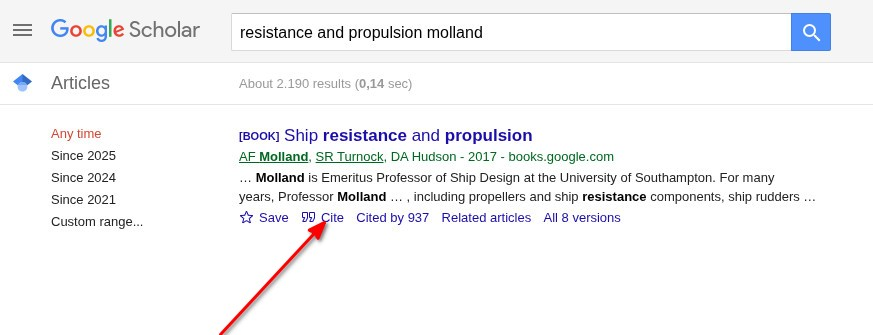
\includegraphics[width=0.8\linewidth]{figs/gs_reference_01.jpg}
	\end{center}
	\caption{Rezultat iskanja v GS}
	\label{fig:gs_cite_01}
\end{figure}

Sedaj izberemo opcijo \texttt{BibTex} in podatke shranimo v našo datoteko\\
\texttt{literatura.bib}, ki se nahaja v isti mapi kakor latex datoteka diplomske naloge.

\begin{figure}[h]
	\begin{center}
		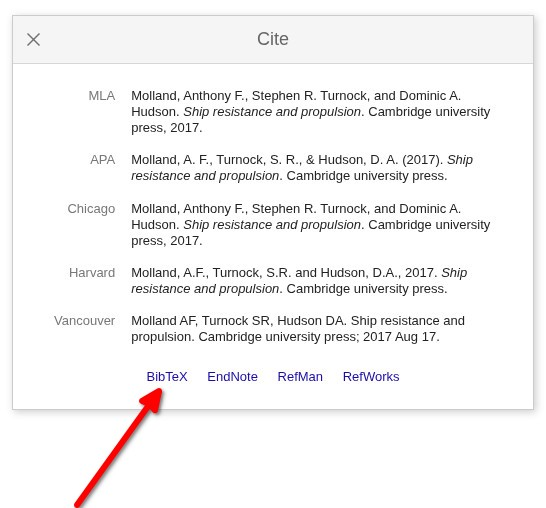
\includegraphics[width=0.8\linewidth]{figs/gs_reference_02.jpg}
	\end{center}
	\caption{Podatki o viru}
	\label{fig:gs_cite_02}
\end{figure}

Podatke označimo in jih skopiramo v datoteko. Zelo preprosto. Vir sedaj citiramo z uporabo ukaza \texttt{cite}, recimo \texttt{\textbackslash cite\{molland2017ship\}} \cite{molland2017ship}.

Potem imamo recimo sklicevanje na več knjig \cite{glob,lang,kalisnik}, in pa referata \cite{zbornik}. V primeru članka z več avtorji \cite{vec-avtorjev} ali pa internetnega vira \cite{wiki} ali \cite{web:lang:stats}.


% ******************
% *** Literatura ***
% ******************
\vkljucibibliografijo{literatura}

\end{document}



